\preamble{Noun}{Noun In English}

\chapter{Overview}
\begin{center}
    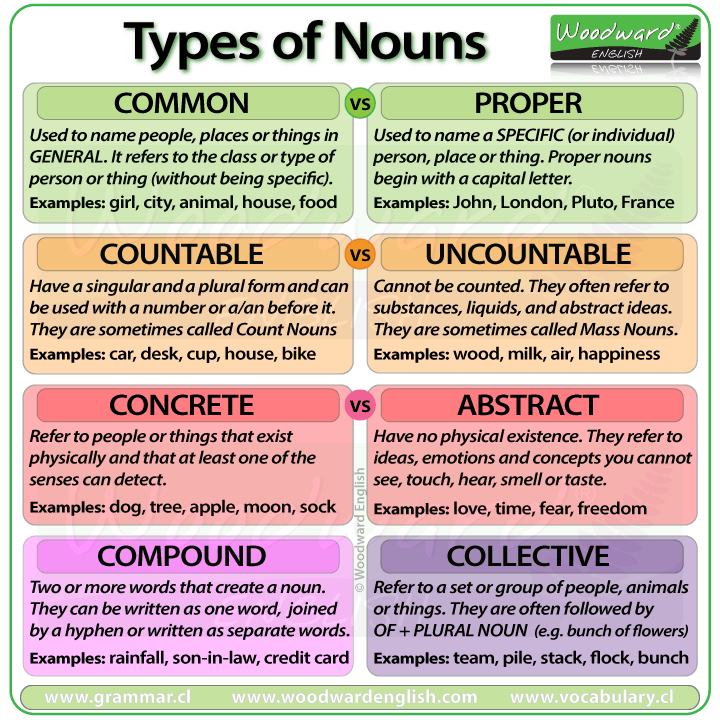
\includegraphics[scale=0.5]{project-folders/Noun/overview.png}
\end{center}

\chapter{Definition}
Nouns refer to persons, animals, places, things, ideas, or events, etc.
Nouns encompass most of the words of a language.\\\\
Noun can be a/an:
\begin{itemize}
    \itembf{Person} – a name for a person: - Max, Julie, Catherine, Michel, Bob, etc.
    \itembf{Animal} – a name for an animal: - dog, cat, cow, kangaroo, etc.
    \itembf{Place} – a name for a place: - London, Australia, Canada, Mumbai, etc.
    \itembf{Thing} – a name for a thing: - bat, ball, chair, door, house, computer, etc.
    \itembf{Idea} – A name for an idea: - devotion, superstition, happiness, excitement, etc.
\end{itemize}

\chapter{Types}
\section{Scale}
\subsection{Proper Noun}
A proper noun is a name which refers only to a single person, place,
or thing and there is no common name for it.
In written English, a proper noun always begins with capital letters.\\\\
\textbf{Example}:
\begin{itemize}
    \itembf{Melbourne} (it refers to only one particular city)
    \itembf{Australia} (there is no other country named Australia; this name is fixed for only one country)
\end{itemize}

\subsection{Common Noun}
A common noun is a name for something which is common for many things, person, or places. It encompasses a particular type of things, person, or places.\\\\
\textbf{Example}: \textbf{Country} (it can refer to any country, nothing in particular)\\\\
So, a common noun is a word that indicates a person, place, thing, etc. In general and a proper noun is a specific one of those

\newpage
\section{Physical Existence}
\subsection{Concrete Noun}
A concrete noun is the exact opposite of abstract noun. It refers to the things we see and have physical existence.\\\\
\textbf{Example}: Chair, table, bat, ball, water, money, sugar, etc.

\subsection{Abstract Noun}
An abstract noun is a word for something that cannot be seen but is there. It has no physical existence. Generally, it refers to ideas, qualities, and conditions.\\\\
\textbf{Example}: Truth, lies, happiness, sorrow, time, friendship, humor, patriotism, etc.

\newpage
\section{Countable}
\subsection{Countable Noun}
The nouns that can be counted are called countable nouns. Countable nouns can take an article: a, an, the.\\\\
\textbf{Example}: Chair, table, bat, ball, etc. (you can say 1 chair, 2 chairs, 3 chairs – so chairs are countable)
\subsection{Attention!}
\textbf{Abstract nouns and proper nouns are always non-countable nouns, but common nouns and concrete nouns can be both count and non-count nouns.}

\subsection{Non-Countable Noun}
The nouns that cannot be counted are called non-countable nouns.\\\\
\textbf{Example}: Water, sugar, oil, salt, etc. (you cannot say “1 water, 2 water, 3 water” because water is not countable)

\newpage
\section{Quantity}
\subsection{Singular Noun}
Singular Nouns are namely, singular in number. The base form of any noun is naturally singular and so that is the Singular Noun.\\\\
\textbf{Examples}: Duck, Bush, Man, Mouse, Child, Fish etc. are Singular Nouns.

\subsection{Plural Noun}
The plural forms of the Singular Nouns are Plural Nouns. These nouns determine more than one element.\\\\
\textbf{Examples}: Belts, Boxes, Mice, Sheep, People etc. are examples of Plural Noun.


\newpage
\subsection{Regular Noun}
Regular Nouns do not change in spelling when changed into plural; only the regular plural suffixes -s or -es are attached to it according to the grammar and spelling agreement.\\\\
\textbf{Examples}:
\begin{tabular}{|c|c|}\hline
    Singular Noun & Plural Noun \\\hline
    Duck          & Ducks       \\\hline
    Belt          & Belts       \\\hline
    Box           & Boxes       \\\hline
    Bush          & Bushes      \\\hline
    Apple         & Apples      \\\hline
\end{tabular}

\subsection{Irregular Noun}
Irregular Nouns do not have plural suffixes added to them for their plural form and they monumentally change in spelling.\\\\
\textbf{Examples}:
\begin{tabular}{|c|c|}\hline
    Singular Noun & Plural Noun \\\hline
    Man           & Men         \\\hline
    Ox            & Oxen        \\\hline
    Fox           & Vixen       \\\hline
    Goose         & Geese       \\\hline
    Mouse         & Mice        \\\hline
\end{tabular}

\newpage
\section{Other}
\subsection{Collective Noun}
A collective noun is a word for a group of things, people, or animals, etc.\\\\
\textbf{Example}: family, team, jury, cattle, etc.\\\\
\textbf{Collective nouns can be both plural and singular. However, Americans prefer to use collective nouns as singular, but both of the uses are correct in other parts of the world.}

\subsection{Compound Noun}
Sometimes two or three nouns appear together, or even with other parts of speech, and create idiomatic compound nouns. Idiomatic means that those nouns behave as a unit and, to a lesser or greater degree, amount to more than the sum of their parts.\\\\
\textbf{Example}: six-pack, five-year-old, and son-in-law, snowball, mailbox, etc.

\newpage
\subsection{Possessive Noun}
The noun that owns something or has something in its possession is the Possessive Noun. These nouns usually end with an apostrophe before one “s” that determines the possession of the object(s) that follows. \\\\
\textbf{Example}:
\begin{itemize}
    \item My cat’s litter needs changing very soon.
    \item Jacky’s wallet is stolen.
    \item Your pet’s feeder is missing.
\end{itemize}

\subsection{Material Noun}
Substances made out of tangible materials are usually Material Nouns. These are Common Uncountable Nouns by nature since they mostly determine a certain sector type of product.\\\\
\textbf{Examples}:
\begin{itemize}
    \item I lack the common fascination with gold.
    \item Coal produces nonrenewable energy.
    \item Humans are 70\% water.
\end{itemize}


\chapter{Functions of Nouns}
Nouns can be used as a subject, a direct object, and an indirect object of a verb; as an object of a preposition; and as an adverb or adjective in sentences. Nouns can also show possession.\\\\

\begin{itemize}
    \itembf{Subject}: The company is doing great.
    \itembf{Direct object}: I finally bought a new mobile.
    \itembf{Indirect object}: Max gave Carol another chocolate.
    \itembf{Object of preposition}: Roses are the flowers of love.
    \itembf{Adverb}: The train leaves today.
    \itembf{Adjective}: The office building faces the mall.
    \itembf{Possession}: The lion’s cage is dangerous.
\end{itemize}